%%%%%%%%%%%%%%%%%%%%%%%%%%%%%%%%%%%%%%%%%
% Thin Sectioned Essay
% LaTeX Template
% Version 1.0 (3/8/13)
%
% This template has been downloaded from:
% http://www.LaTeXTemplates.com
%
% Original Author:
% Nicolas Diaz (nsdiaz@uc.cl) with extensive modifications by:
% Vel (vel@latextemplates.com)
%
% License:
% CC BY-NC-SA 3.0 (http://creativecommons.org/licenses/by-nc-sa/3.0/)
%
%%%%%%%%%%%%%%%%%%%%%%%%%%%%%%%%%%%%%%%%%

%----------------------------------------------------------------------------------------
%	PACKAGES AND OTHER DOCUMENT CONFIGURATIONS
%----------------------------------------------------------------------------------------

\documentclass[a4paper, 11pt]{article} % Font size (can be 10pt, 11pt or 12pt) and paper size (remove a4paper for US letter paper)

\usepackage[protrusion=true,expansion=true]{microtype} % Better typography
\usepackage{graphicx} % Required for including pictures
\usepackage[utf8]{inputenc}
\usepackage[spanish]{babel}
\usepackage{mathpazo} % Use the Palatino font
\usepackage[T1]{fontenc} % Required for accented characters
\linespread{1.05} % Change line spacing here, Palatino benefits from a slight increase by default

\makeatletter
\renewcommand\@biblabel[1]{\textbf{#1.}} % Change the square brackets for each bibliography item from '[1]' to '1.'
\renewcommand{\@listI}{\itemsep=0pt} % Reduce the space between items in the itemize and enumerate environments and the bibliography

\renewcommand{\maketitle}{ % Customize the title - do not edit title and author name here, see the TITLE block below
\begin{flushright} % Right align
{\LARGE\@title} % Increase the font size of the title

\vspace{50pt} % Some vertical space between the title and author name

{\large\@author} % Author name
\\\@date % Date

\vspace{40pt} % Some vertical space between the author block and abstract
\end{flushright}
}

%----------------------------------------------------------------------------------------
%	TITLE
%----------------------------------------------------------------------------------------

\title{\textbf{Práctica 1}\\ % Title
Análisis de eficiendia de algoritmos} % Subtitle

\author{\textsc{Francisco Carrillo Pérez,Borja Cañavate Bordons, Miguel Porcel Jiménez,Jose Manuel Rejón Santiago,Jose Arcos Aneas } % Author
\\{\textit{Universidad de Granada}}} % Institution

\date{\today} % Date

%----------------------------------------------------------------------------------------

\begin{document}

\maketitle % Print the title section

%----------------------------------------------------------------------------------------
%	ABSTRACT AND KEYWORDS
%----------------------------------------------------------------------------------------

%\renewcommand{\abstractname}{Summary} % Uncomment to change the name of the abstract to something else

\begin{abstract}
Vamos a realizar el análisis de eficiencia empírico e híbrido varias algoritmos, comparando los resultados experimentales con el valor
teórico que deberían dar. Incluiremos gráficas para que se vea la clara diferencia entre ambos.
\end{abstract}

\vspace{30pt} % Some vertical space between the abstract and first section

%----------------------------------------------------------------------------------------
%	ESSAY BODY
%----------------------------------------------------------------------------------------

\section{Introducción }
\begin{frame}
	
	\begin{itemize}
		\item El objetivo de ésta práctica es analizar eficiencias de forma empírica e híbrida.
		\item Para ello, hemos recogido los diferentes tiempos de los diferentes algoritmos que se ofrecían y los hemos comparado.
		\item En nuestro caso concreto, hemos utilizado la biblioteca de C++ más moderna y precisa destinado a obtener tiempos de reloj: la biblioteca \textbf{chrono}
	\end{itemize}
\end{frame}
\begin{frame}
	
	\begin{itemize}
		
		\item Procesador: Intel Core i5-3337U (2.7GHz x 2)
		\item Memoria RAM: 4GB
		\item Disco Duro: 500GB 5400 rpm
		\item SO: Manjaro Linux 15.2 Capella 64 bits
	\end{itemize}
	
\end{frame}


%------------------------------------------------
\section{Ordenación} % Sections can be created in order to organize your presentation into discrete blocks, all sections and subsections are automatically printed in the table of contents as an overview of the talk
%------------------------------------------------

	
	Según hemos ido hemos estudiado, estos algoritmos que presentamos tienen teóricamente y calculando a partir del código una eficiencia de $O(n^2 )$. Como esto es teórico, vamos a ver si efectivamente (o no) los algoritmos proporcionados se parecen a la gráfica de $n^2$ recogiendo la información de 99 posibilidades distintas en cada algoritmo.
	\begin{figure}[htb]
		\centering
		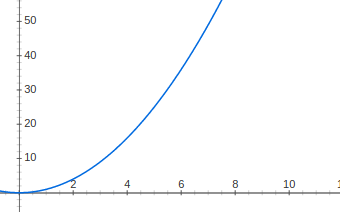
\includegraphics[width=0.5\linewidth]{imagenes/enecuadrado.png}
		\caption{Gráfica de la función $n^2$}
		\label{fig:E1}
	\end{figure}
	


\subsection{Burbuja}

	
	La gráfica empírica obtenida ha sido:
	\begin{figure}[htb]
		\centering
		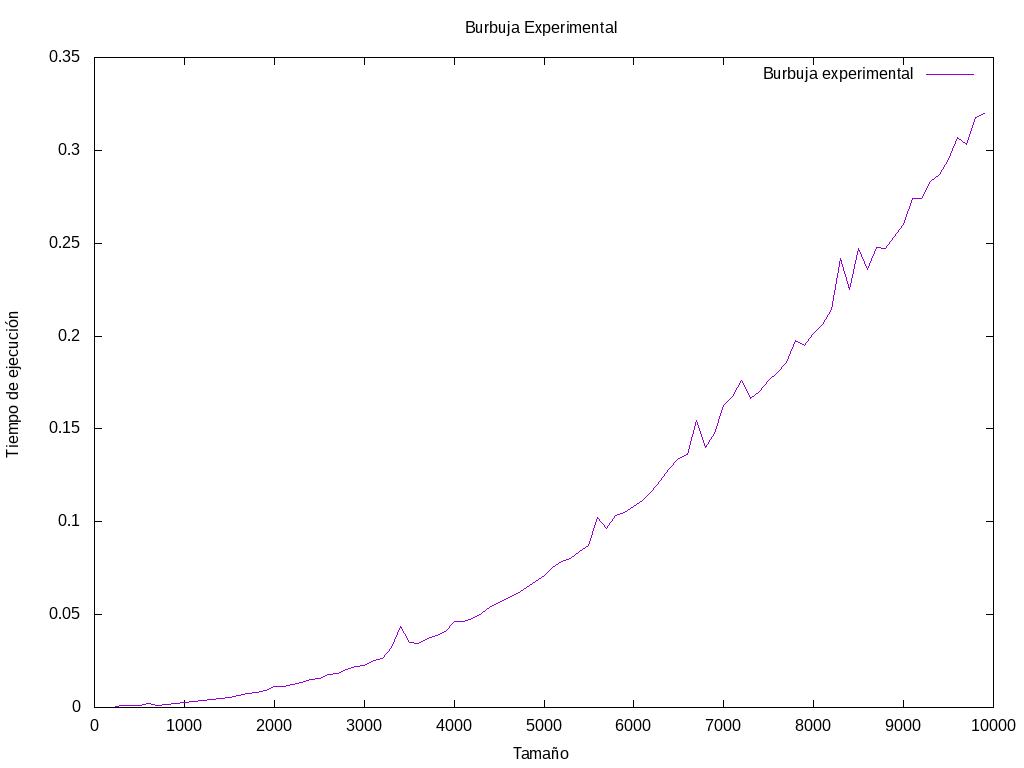
\includegraphics[width=0.7\linewidth]{imagenes/burbuja-experimental.png}
		\caption{Algoritmo de Burbuja, gráfica empírica.}
		\label{fig:E2}
	\end{figure}
	




	La gráfica híbrida obtenida ha sido:
	\begin{figure}[htb]
		\centering
		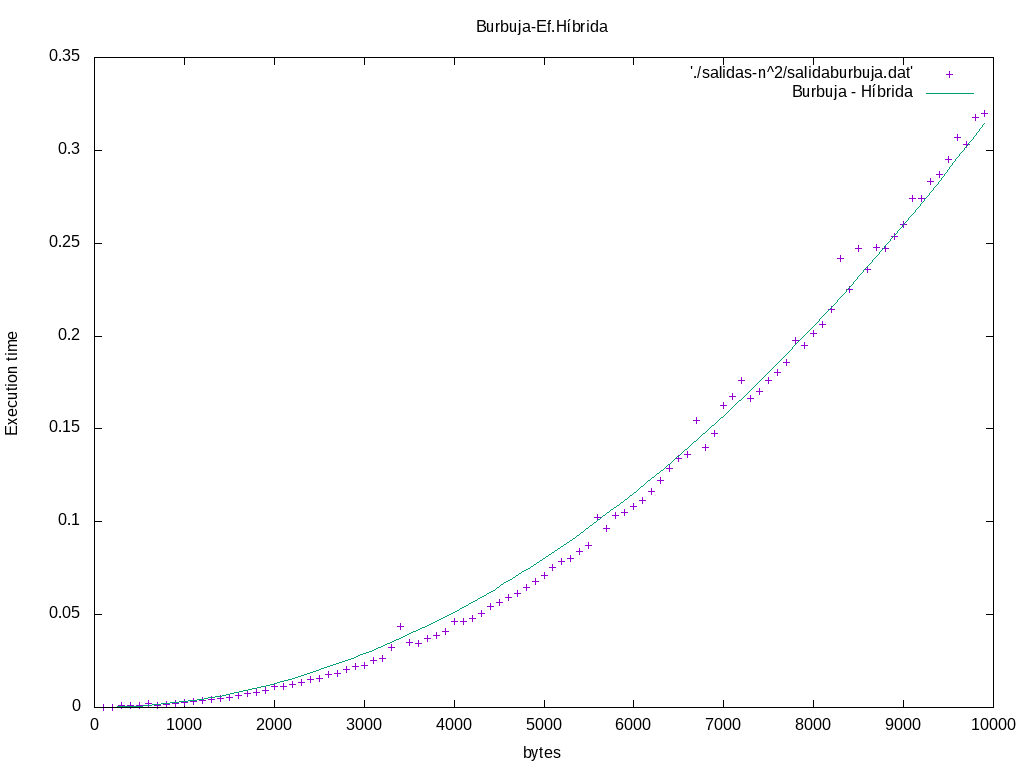
\includegraphics[width=0.7\linewidth]{imagenes/burbuja-hibrida.png}
		\caption{Ajuste híbrido algoritmo Burbuja y función $n^2$}
		\label{fig:E3}
	\end{figure}	






\subsection{Selección}

	
	La gráfica empírica obtenida ha sido:
	\begin{figure}[htb]
		\centering
		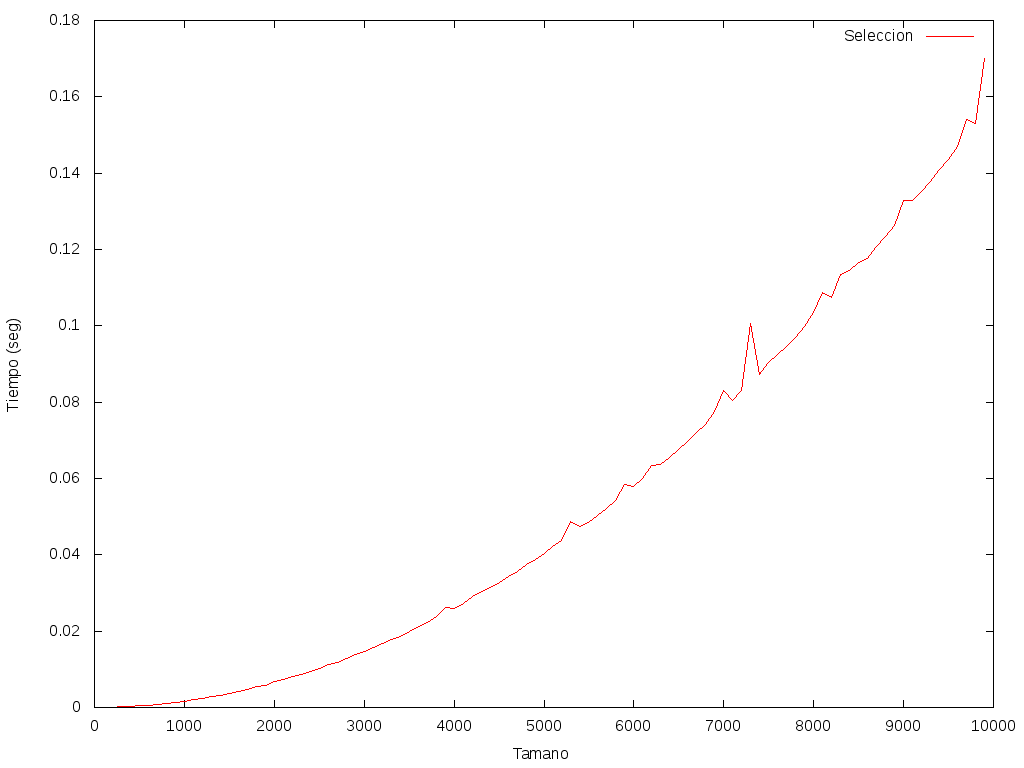
\includegraphics[width=0.7\linewidth]{imagenes/seleccionLines.png}
		\caption{Algoritmo de selección, gráfica empírica. }
		\label{fig:E4}
	\end{figure}



	
	La gráfica híbrida obtenida ha sido:
	\begin{figure}[htb]
		\centering
		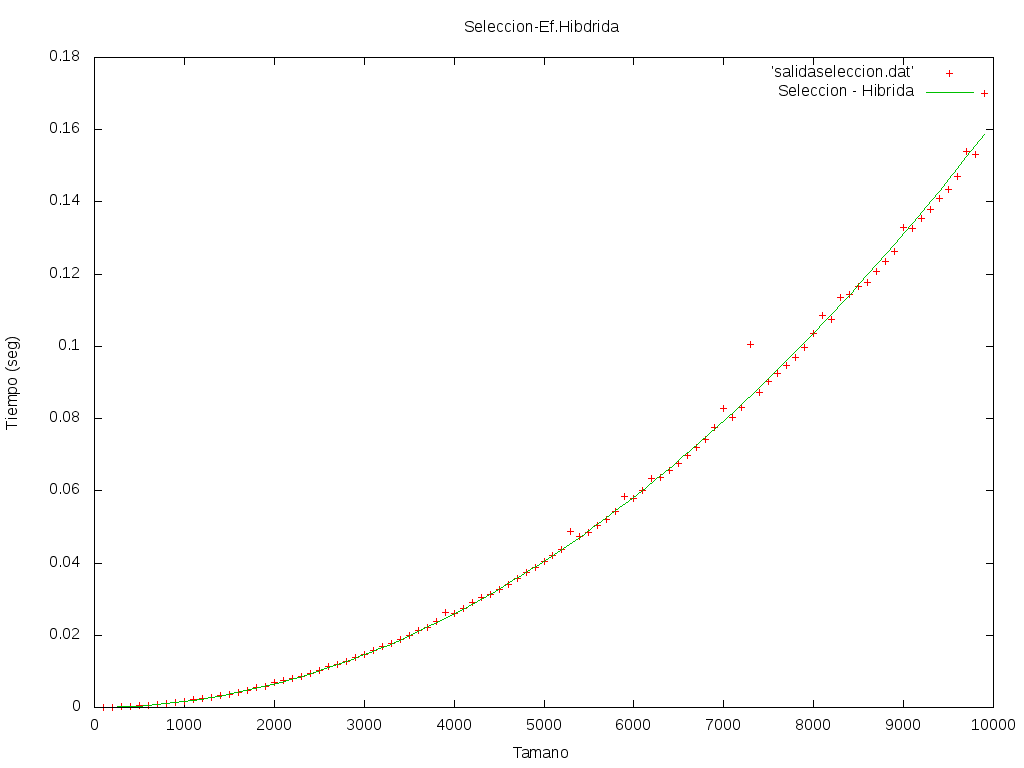
\includegraphics[width=0.7\linewidth]{imagenes/seleccion-hibrida.png}
		\caption{Gráfica ajuste híbrido. Selección y $n^2$}
		\label{fig:E5}
	\end{figure}
	

\subsection{Inserción}

La gráfica empírica obtenida ha sido:
\begin{figure}[htb]
	\centering
	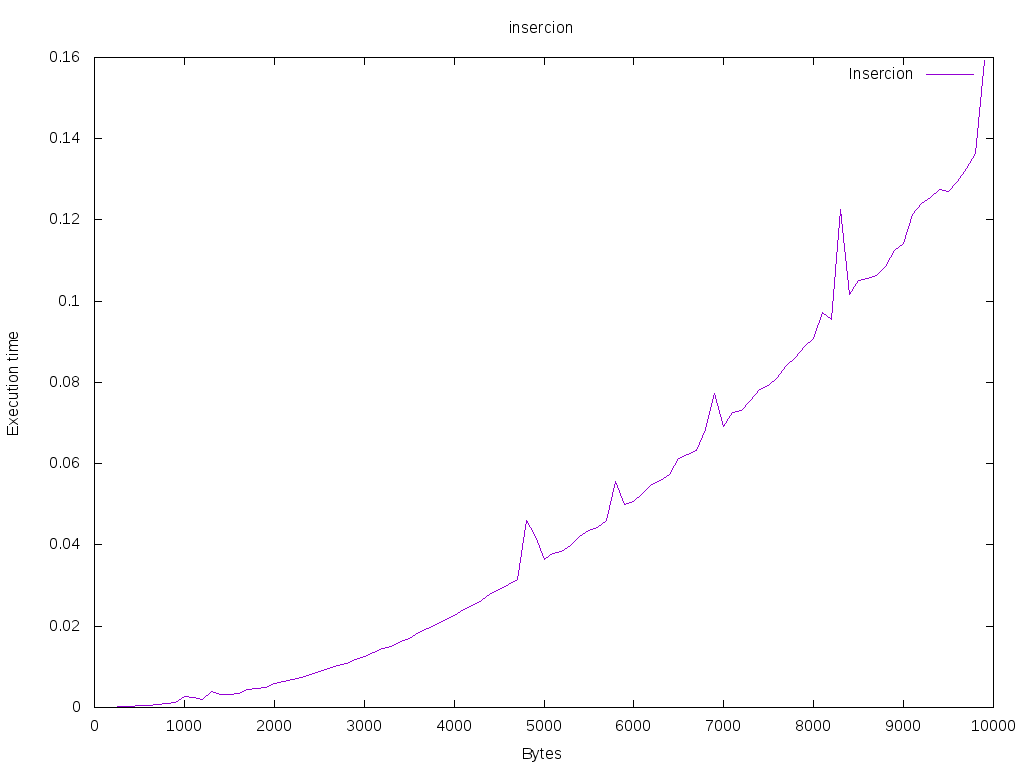
\includegraphics[width=0.7\linewidth]{imagenes/insercion.png}
	\caption{Algoritmo de Inserción, gráfica empírica.}
	\label{fig:E6}
\end{figure}
	

La gráfica híbrida obtenida ha sido:
\begin{figure}[htb]
	\centering
	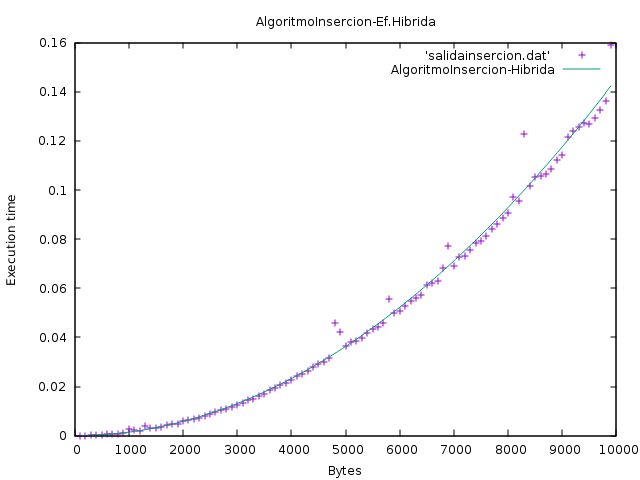
\includegraphics[width=0.7\linewidth]{imagenes/algoritmoInsercion-hibrida}
	\caption{Gráfica ajuste híbrido. Inserción y $n^2$}
	\label{fig:E7}
\end{figure}
Por último, mostramos el porcentaje de error así como las constantes ocultas obtenidas.\\
\begin{center}
	\begin{tabular}{| l | c | r |}
		\hline
		\textbf{Algoritmo} & \textbf{Constante Oculta} & \textbf{Error} \\
		\hline
		Burbuja & a0 = 3.20873e-09 & +/- 1.403e-11 (0.4372\%)\\ \hline
		Selección & a0 = 1.61988e-09 & +/- 4.818e-12 (0.2975\%) \\ \hline		
		Inserción & a0 = 1.45151e-09 &  +/- 8.337e-12    (0.5743\%) \\ \hline
	\end{tabular}
\end{center}
	
	
\section{Ordenación rápida} % Sections can be crea es muy bajoted in order to organize your presentation into discrete blocks, all sections and subsections are automatically printed in the table of contents as an overview of the talk
%------------------------------------------------
Según hemos ido estudiado, estos algoritmos que presentamos tienen teóricamente y calculando a partir del código una eficiencia de $O(n*\log(n) )$. Como esto es teórico, vamos a ver si efectivamente (o no) los algoritmos proporcionados se parecen a la gráfica de $n*\log(n)$ recogiendo la información de 99 posibilidades distintas en cada algoritmo.
\begin{figure}[htb]
	\centering
	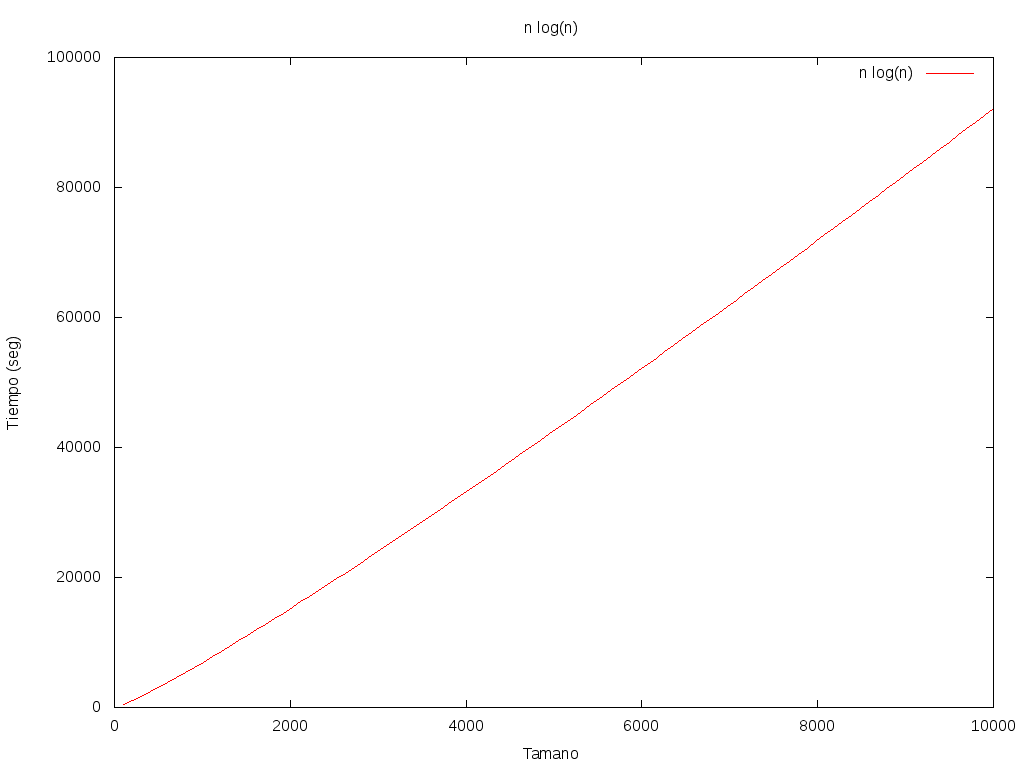
\includegraphics[width=0.5\linewidth]{imagenes/nlog(n)3.png}
	\caption{Gráfica de la función $n*log(n)$}
	\label{fig:E8}
\end{figure}
\subsection{Quick Sort}
La gráfica empírica obtenida ha sido:
\begin{figure}[htb]
	\centering
	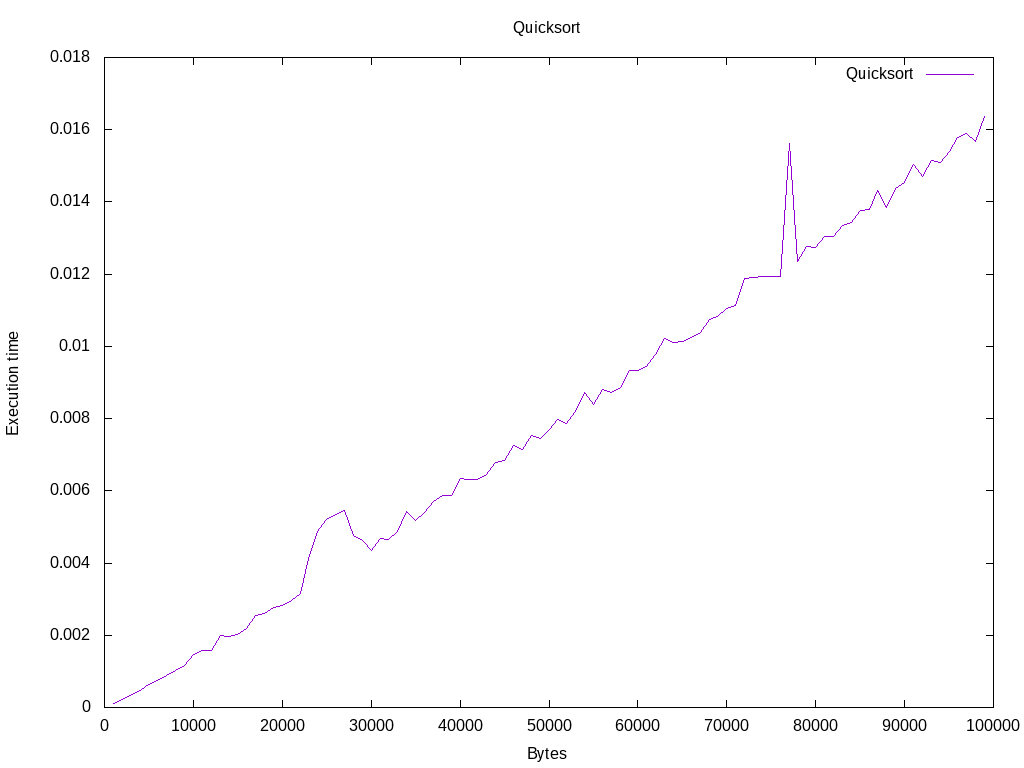
\includegraphics[width=0.7\linewidth]{imagenes/quicksort.png}
	\caption{Algoritmo Quicksort, gráfica empírica. }
	\label{fig:E9}
\end{figure}
	
La gráfica híbrida obtenida ha sido:
\begin{figure}[htb]
	\centering
	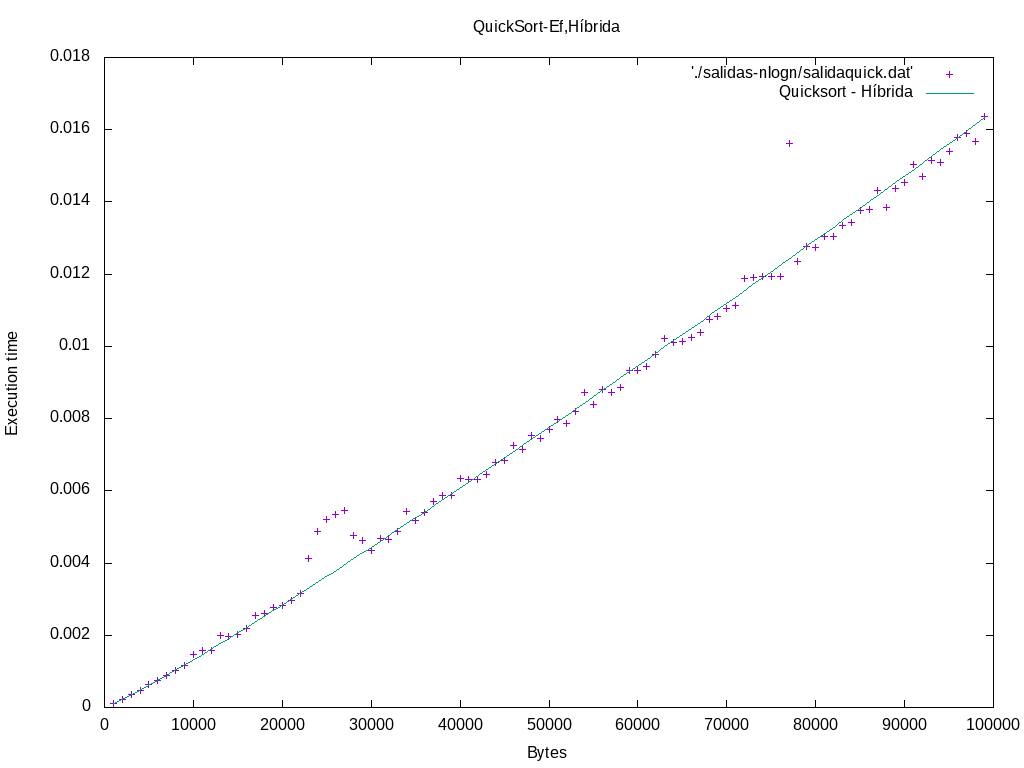
\includegraphics[width=0.7\linewidth]{imagenes/quicksort-hibrida.png}
	\caption{Gráfica híbrida Quicksort.}
	\label{fig:E10}
\end{figure}

\subsection{Heap Sort}
La gráfica empírica obtenida ha sido:
\begin{figure}[htb]
	\centering
	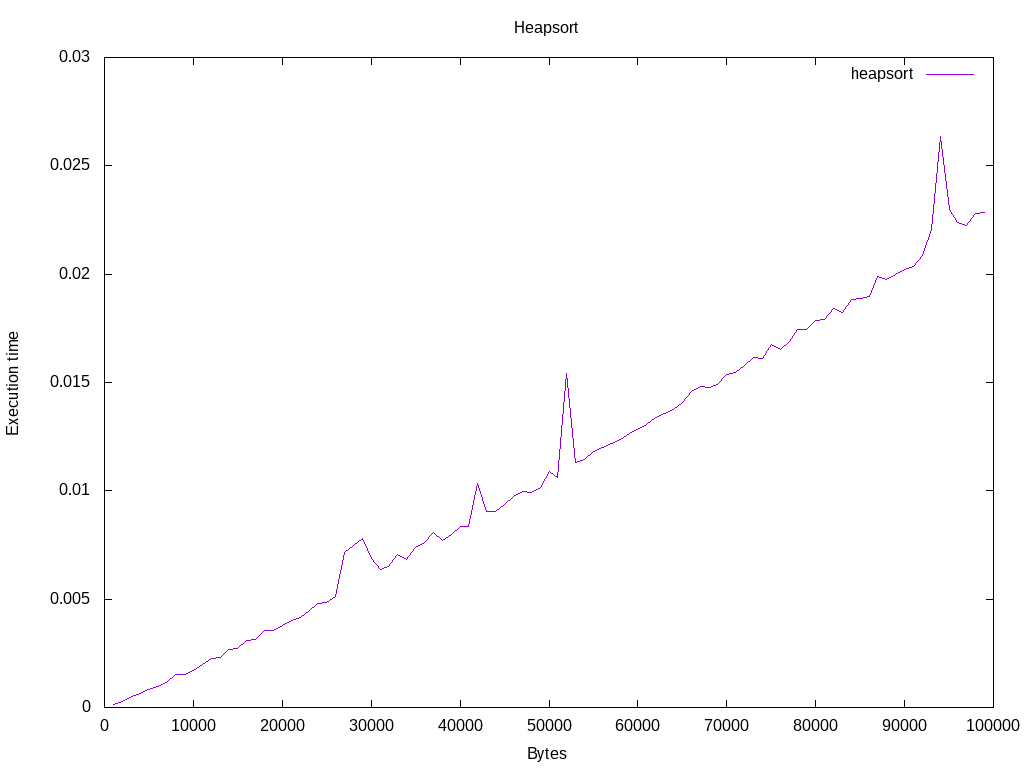
\includegraphics[width=0.7\linewidth]{imagenes/heapsort.png}
	\caption{Heapsort, gráfica empírica.}
	\label{fig:E11}
\end{figure}
	
La gráfica híbrida obtenida ha sido:
\begin{figure}[htb]
	\centering
	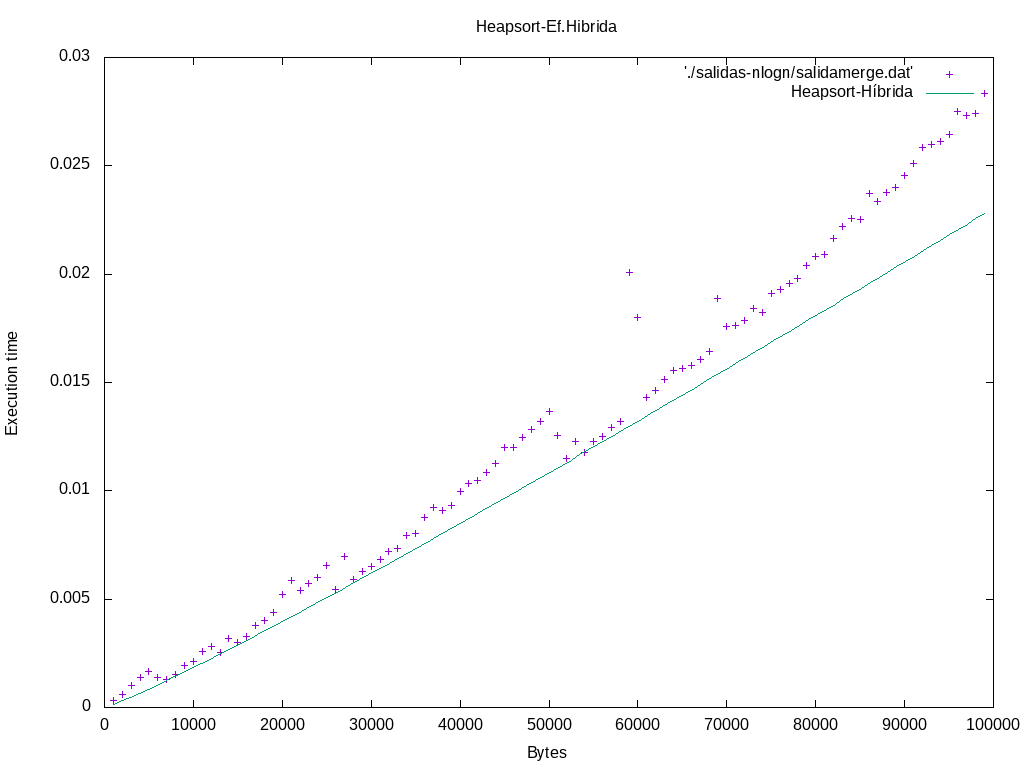
\includegraphics[width=0.7\linewidth]{imagenes/heapsort-hibrida.png}
	\caption{Heapsort, gráfica híbrida.}
	\label{fig:E12}
\end{figure}
Este algoritmo lo hemos ejecutado en otra máquina más potente, de esta manera, podemos ver como varían los tiempos de ejecución del mismo algoritmo, ejecutado en dos máquinas distintas.
\begin{itemize}
	\item Procesador (frecuencia): Intel Core i7-5500U (3.0 GHz x 2)
	\item Memoria RAM: 4 GB
	\item Disco duro: SSD 256 GB
	\item S.O: Linux Mint 17.3 Cinnamon 64-bit
\end{itemize}
El ajuste de ambas gráficas es el siguiente:
\begin{figure}[htb]
	\centering
	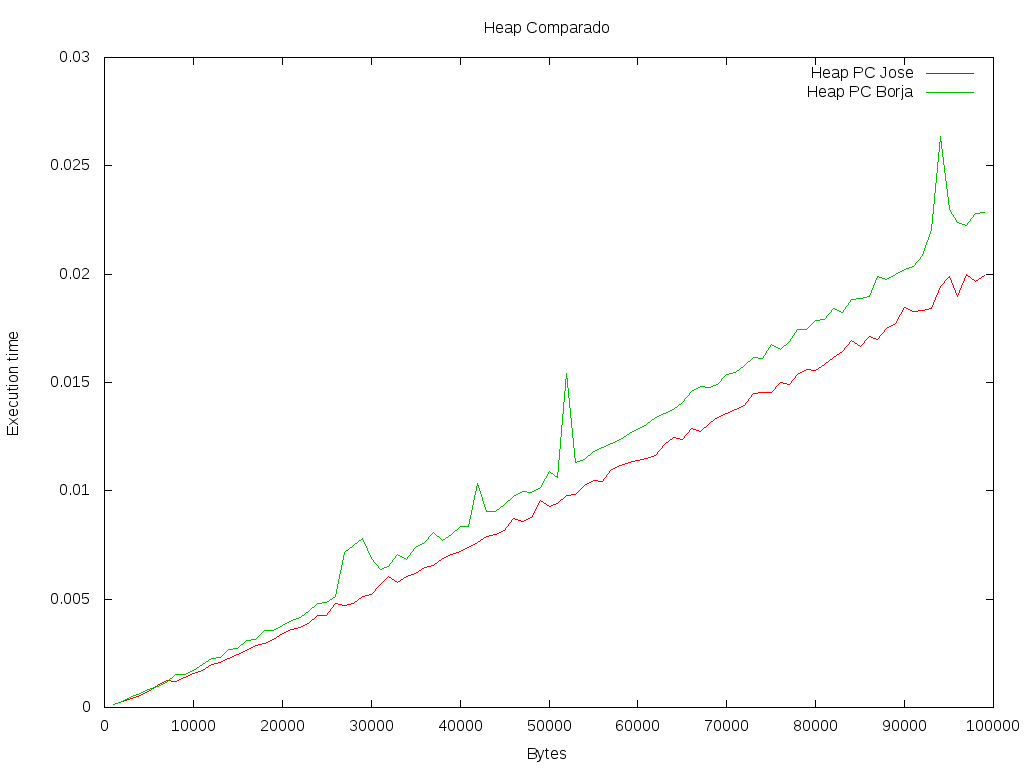
\includegraphics[width=0.7\linewidth]{imagenes/HeapComparado.png}
	\caption{Comparación en dos máquinas. Heapsort.}
	\label{fig:E13}
\end{figure}

\subsection{Merge Sort}
La gráfica empírica obtenida ha sido:
\begin{figure}[htb]
	\centering
	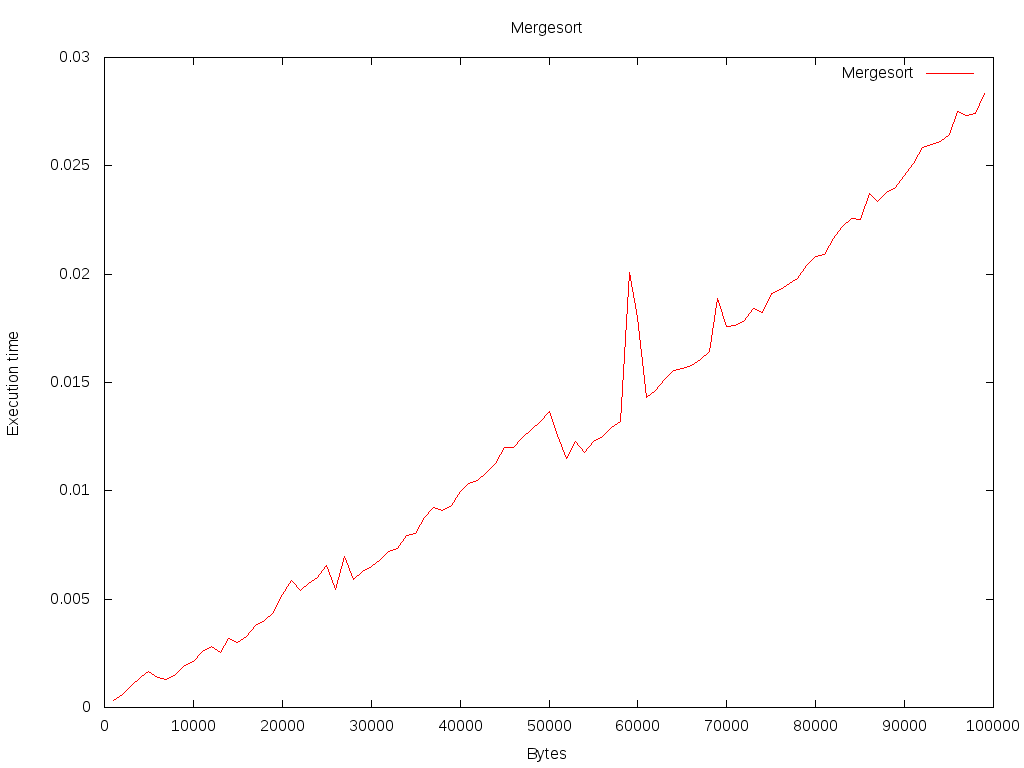
\includegraphics[width=0.7\linewidth]{imagenes/mergesort.png}
	\caption{Mergesort, gráfica empírica.}
	\label{fig:E14}
\end{figure}
La gráfica híbrida obtenida ha sido:
\begin{figure}[htb]
	\centering
	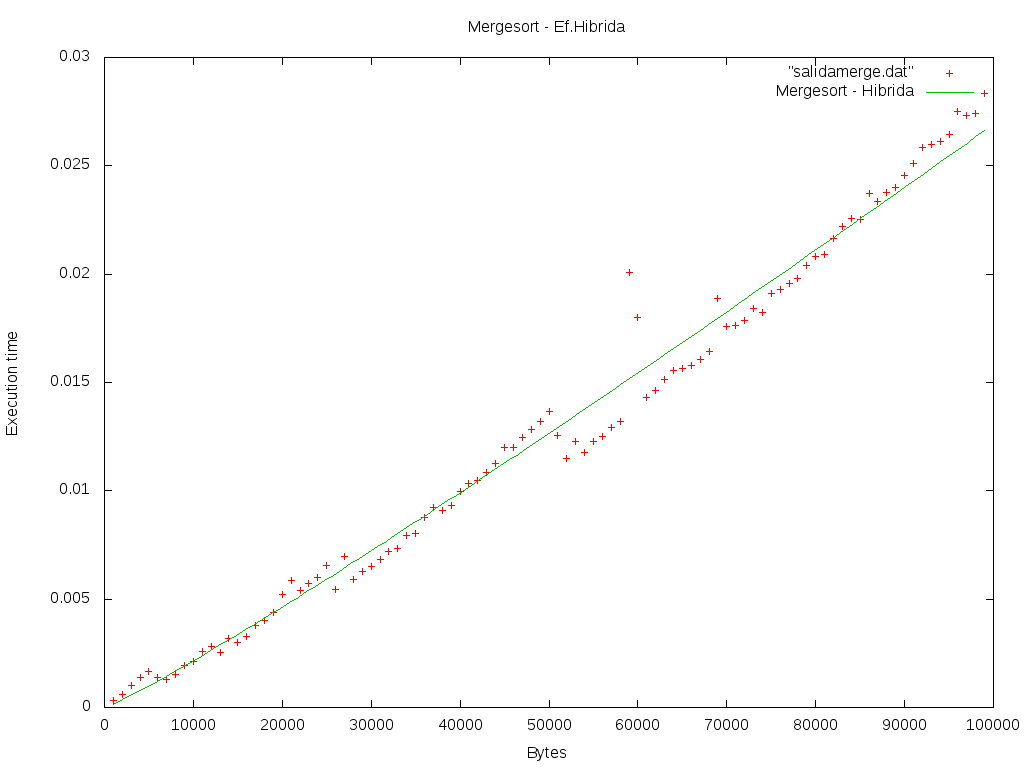
\includegraphics[width=0.7\linewidth]{imagenes/mergesort-hibrida.png}
	\caption{Mergesort, gráfica híbrida.}
	\label{fig:E15}
\end{figure}
Por último, mostramos el porcentaje de error así como las constantes ocultas.\\
\begin{center}
	\begin{tabular}{| l | c | r |}
		\hline
		\textbf{Algoritmo} & \textbf{Constante Oculta} & \textbf{Error} \\ \hline
		Mergesort & a0 = 2.33821e-08 & +/- 1.564e-10 (0.6689\%)\\ \hline
		Quicksort & a0 = 1.43368e-08 & +/- 7.621e-11 (0.5315\%) \\ \hline
		Heapsort & a0 = 2.00227e-08 & +/- 1.222e-10    (0.6104\%) \\ \hline
	\end{tabular}
\end{center}
	
\section{Floyd}

El algoritmo de Floyd, a diferencia de los anteriores, no es un algoritmo de ordenación. Su función, es la de encontrar el camino mínimo en grafos. La eficiencia teórica de este algoritmo es $O(n^3)$. Además de analizar la eficiencia empírica e híbrida, hemos realizado un ajuste erróneo, para demostrar que efectivamente la eficiencia de este algoritmo es la anteriormente mencionada.

\subsection{Gráficas}
\textbf{Gráfica Empírica}\\
\\
La gráfica empírica obtenida ha sido:
\begin{figure}[htb]
	\centering
	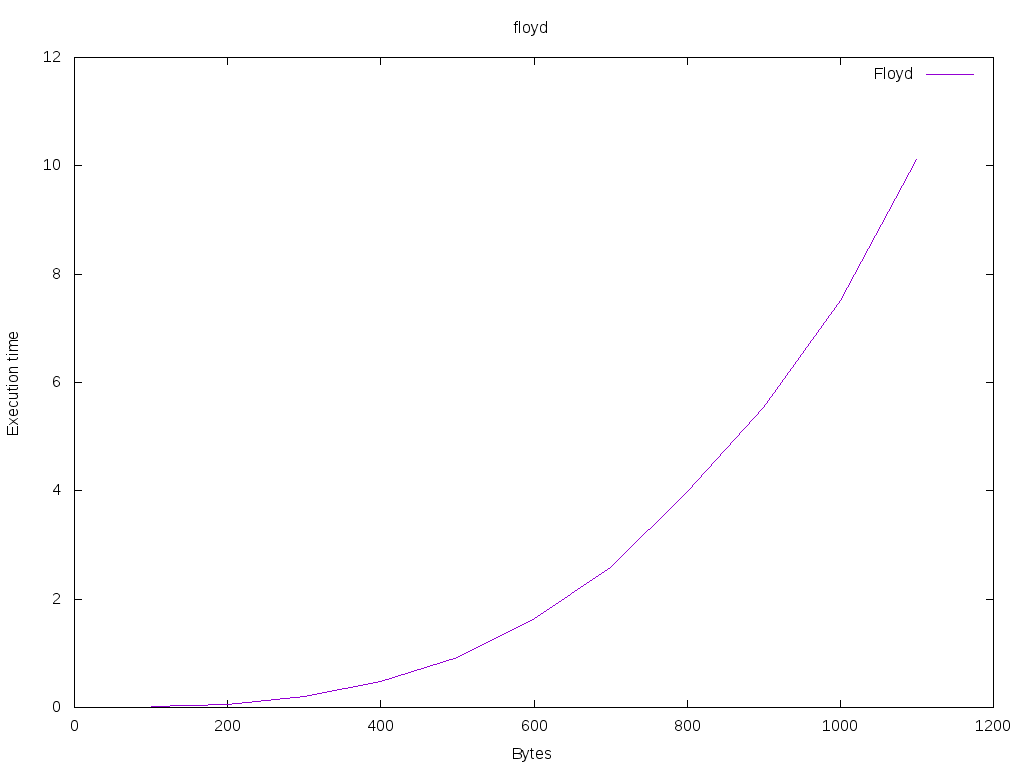
\includegraphics[width=0.7\linewidth]{imagenes/floyd.png}
	\caption{Floyd, gráfica empírica.}
	\label{fig:E16}
\end{figure}
	


\textbf{Gráfica Híbrida}\\
\\
La gráfica híbrida obtenida ha sido:
\begin{figure}[htb]
	\centering
	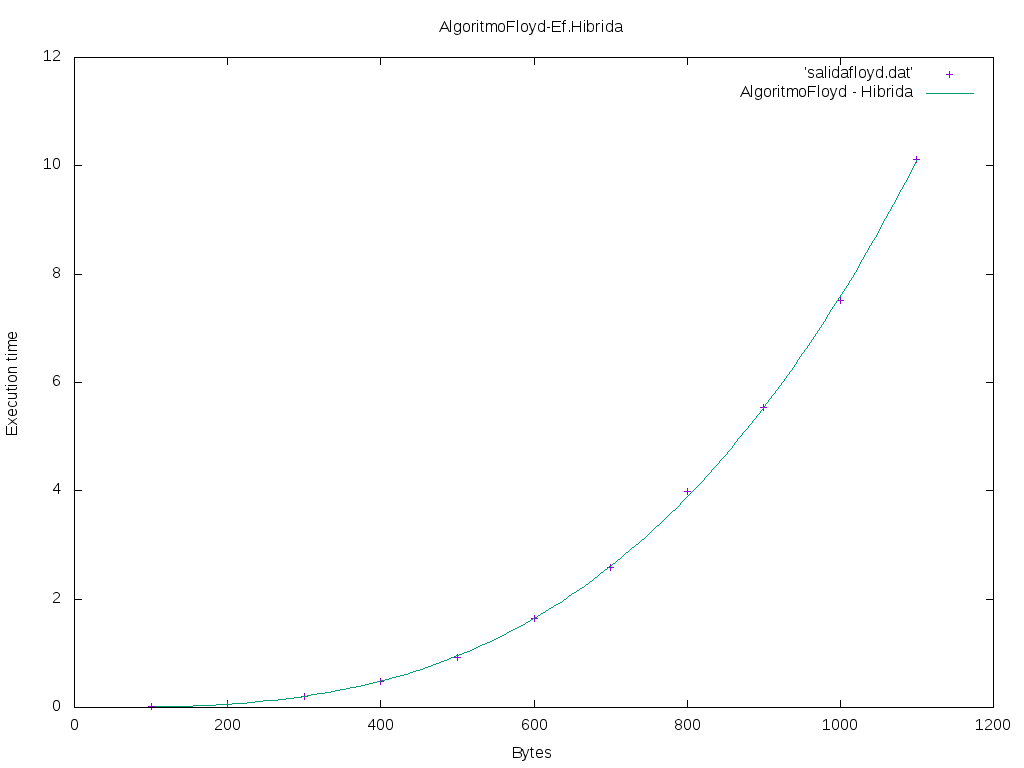
\includegraphics[width=0.7\linewidth]{imagenes/algoritmoFloyd-hibrida.png}
	\caption{Floyd, gráfica híbrida.}
	\label{fig:E17}
\end{figure}


\textbf{Ajuste Híbrido Erróneo}\\
\\
	
Ajuste híbrido erróneo ($O(n^3)$ ajustada a una función $O(n * log(n))$.
\begin{figure}[htb]
	\centering
	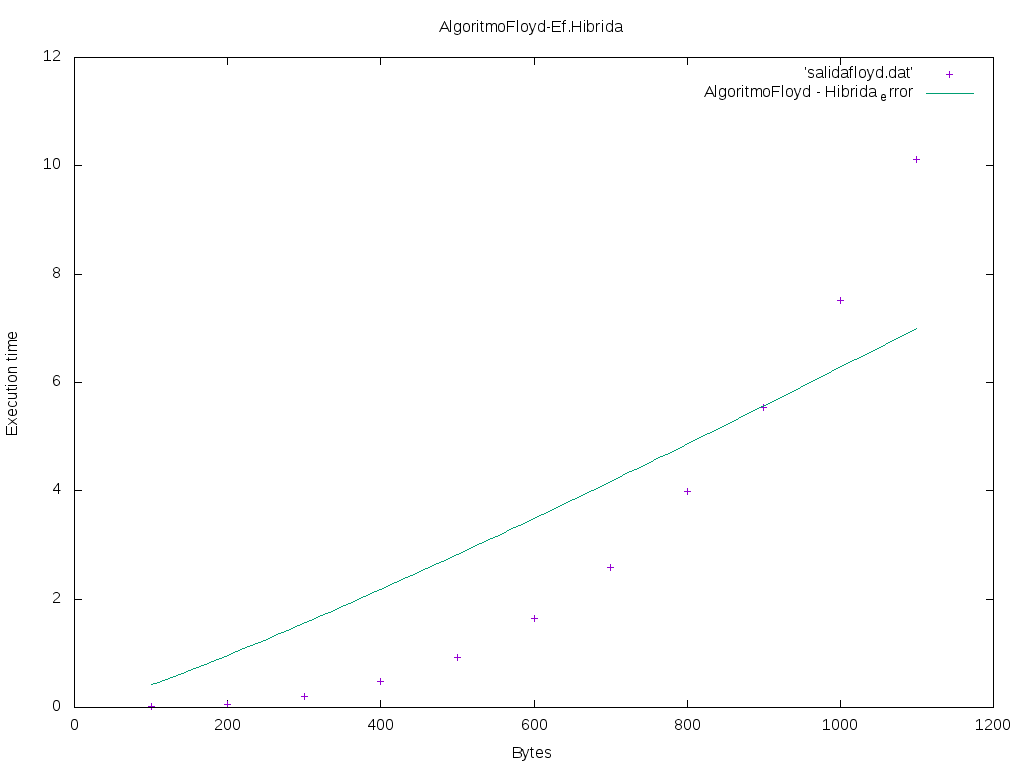
\includegraphics[width=0.7\linewidth]{imagenes/FloydError.png}
	\caption{Floyd, ajuste erróneo.}
	\label{fig:E18}
\end{figure}


\subsection{Porcentaje de error y constantes ocultas}
Por último, mostramos el porcentaje de error así como las constantes ocultas de ambos ajustes.\\
	
\begin{center}
	\begin{tabular}{| l | c | r |}
		\hline
		\textbf{Algoritmo} & \textbf{Constante Oculta} & \textbf{Error} \\ \hline
		Floyd & a0 = 7.59068e-09 & +/- 2.163e-11    (0.2849\%)\\ \hline
		Floyd erróneo & a0 = 0.000908818 & +/- 0.0001093 (12.03\%) \\ \hline
	\end{tabular}
\end{center}
	


\section{Hanoi}

El algoritmo de Hanoi, se encarga específicamente de resolver el problema de las torres de Hanoi. Este algoritmo presenta una eficiencia teórica de $O(2^n)$, lo que hace que el número de entradas para este algoritmo sea muy reducido.

\subsection{Gráficas}
La gráfica empírica obtenida ha sido:
\begin{figure}[htb]
	\centering
	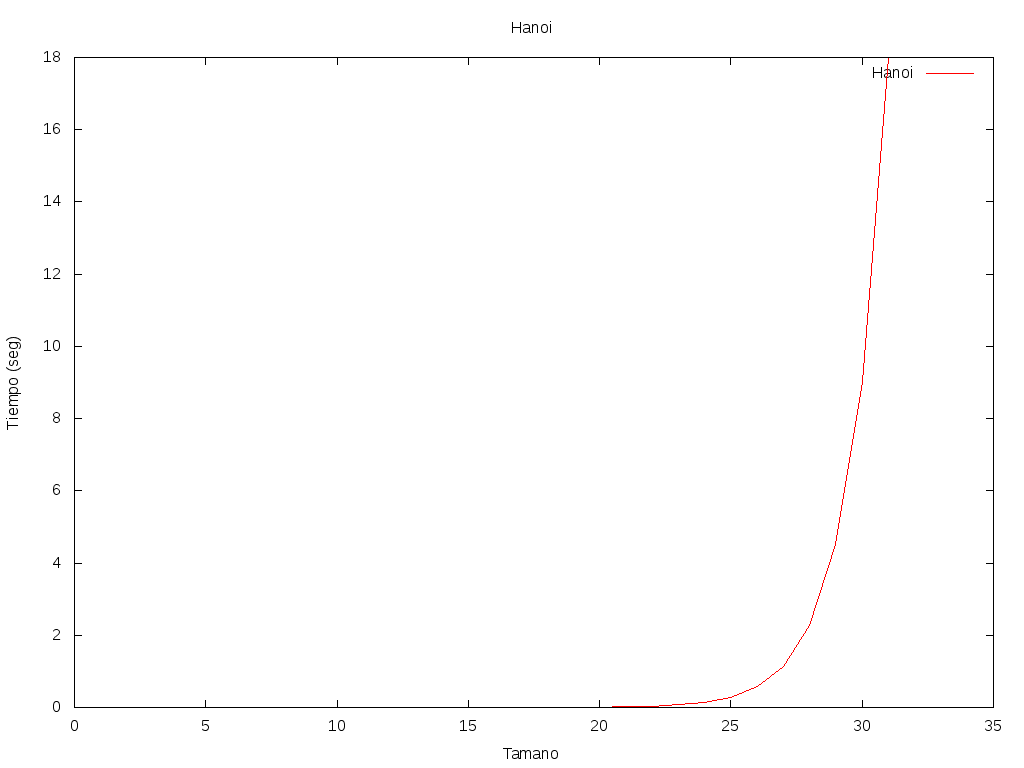
\includegraphics[width=0.7\linewidth]{imagenes/hanoiLines.png}
	\caption{Hanoi, gráfica empírica.}
	\label{fig:E19}
\end{figure}
	
La gráfica híbrida obtenida ha sido:
\begin{figure}[htb]
	\centering
	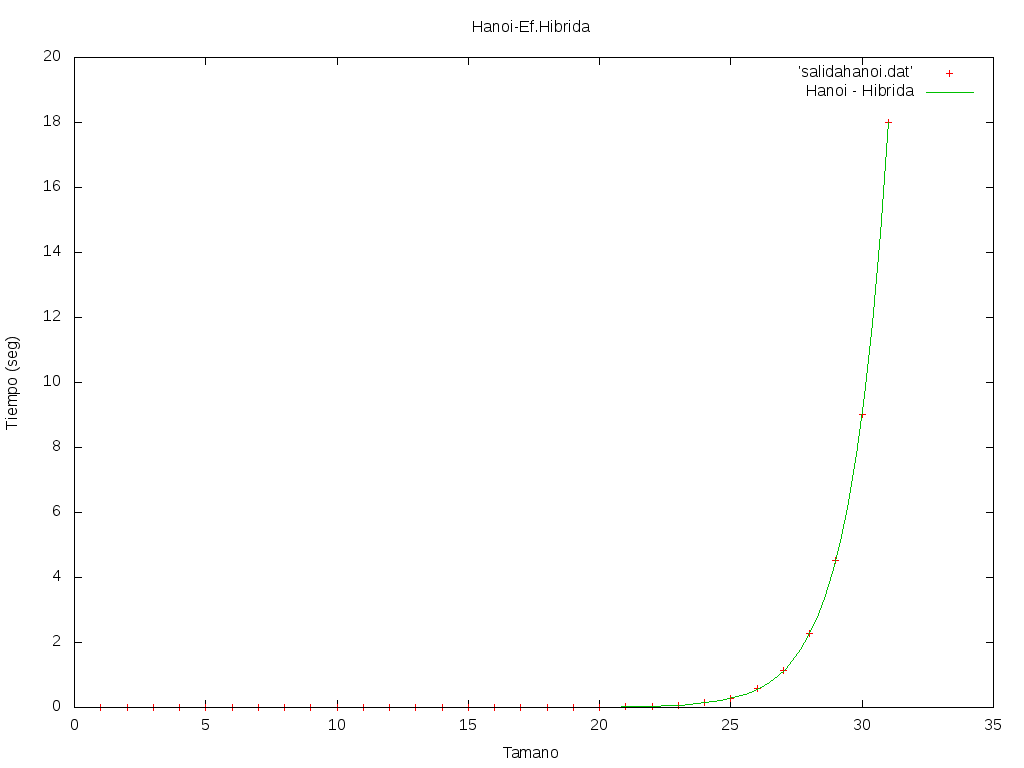
\includegraphics[width=0.7\linewidth]{imagenes/hanoi-hibrido.png}
	\caption{Hanoi, gráfica híbrida.}
	\label{fig:E20}
\end{figure}



\subsection{Comparaciones}
En este algoritmo hemos hecho varias comparaciones:
\begin{itemize}
	\item Usando diferentes optimizaciones a la hora de compilar.
	\item Utilizando un lenguaje de programación distinto (Python vs C++).
\end{itemize}

\subsection{Hanoi en Python}
La gráfica híbrida de la ejecución en Python frente a la ejecución en C++ es:
\begin{figure}[htb]
	\centering
	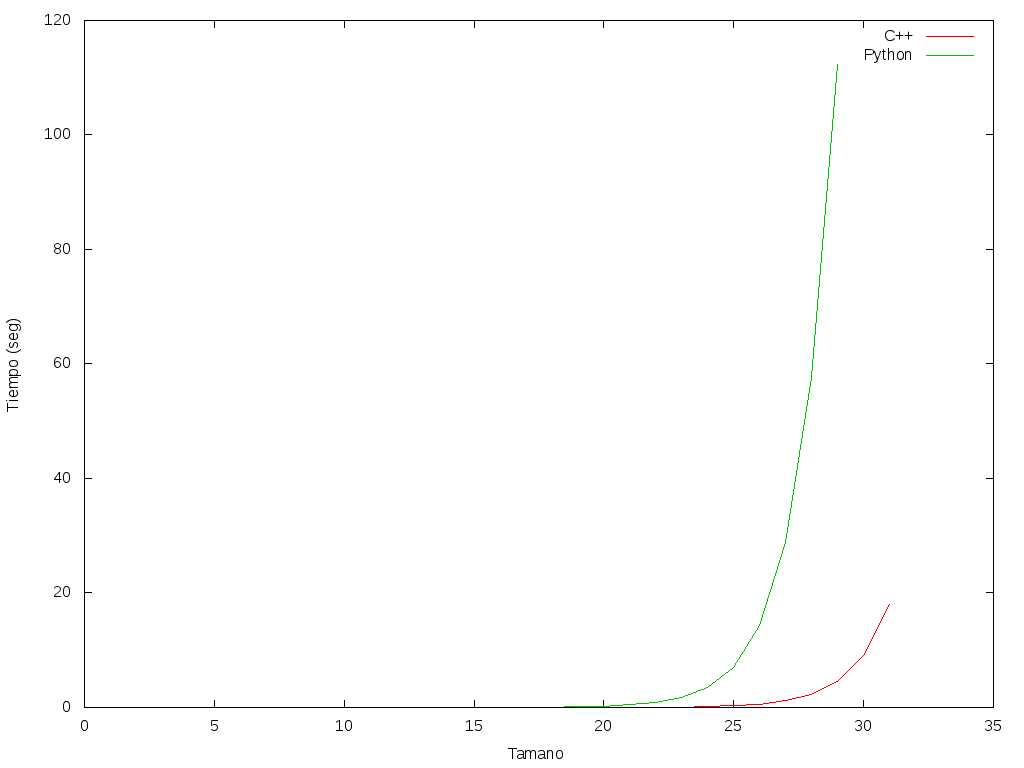
\includegraphics[width=0.7\linewidth]{imagenes/HanoiPy.png}
	\caption{Hanoi, Python - C++}
	\label{fig:E21}
\end{figure}



\subsection{Hanoi con diferentes optimizaciones}
A continuación mostramos una gráfica con los tiempos del algoritmo en función de su optimización:
\begin{figure}[htb]
	\centering
	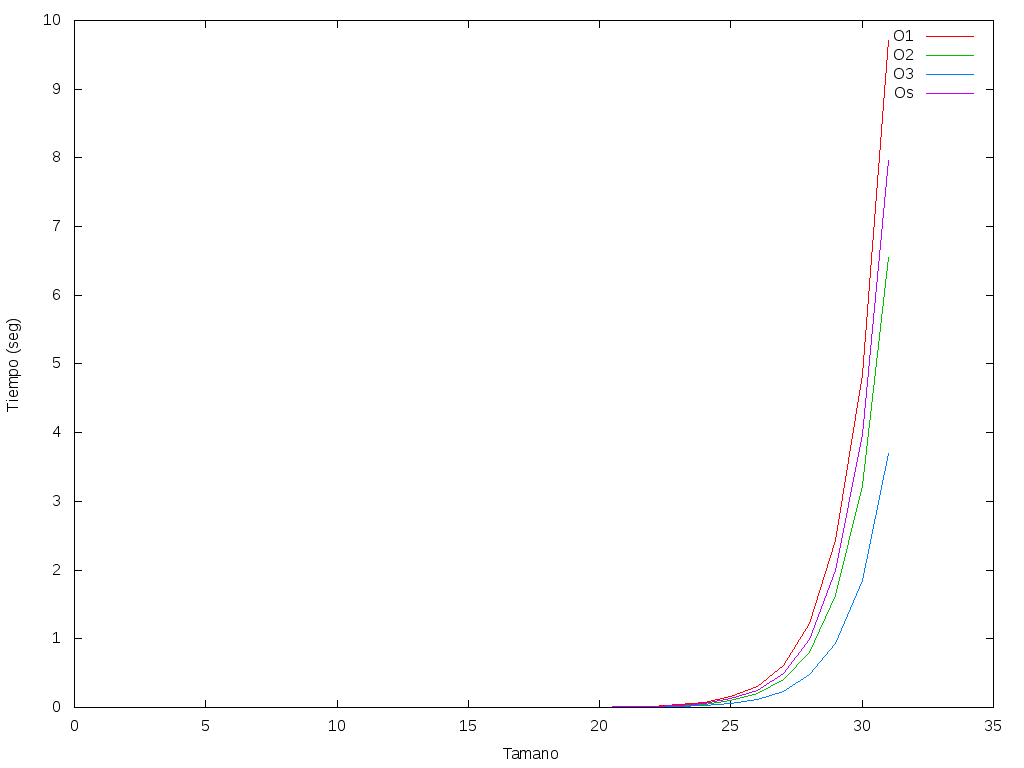
\includegraphics[width=0.7\linewidth]{imagenes/HanoiComparacion.png}
	\caption{Hanoi, gráfica con diferentes eficiencias.}
	\label{fig:E22}
\end{figure}



\subsection{Porcentaje de error y constantes ocultas}
Por último, mostramos el porcentaje de error así como las constantes ocultas.\\
\begin{center}
	\begin{tabular}{| l | c | r |}
		\hline
		\textbf{Algoritmo} & \textbf{Constante Oculta} & \textbf{Error} \\ \hline
		Hanoi & a0 = 8.38461e-09 & +/- 3.095e-12    (0.03691\%)\\ \hline
	\end{tabular}
\end{center}
	

%----------------------------------------------------------------------------------------

\end{document}